%% Stellarium User Guide
% Status:
% 2016-01-03 Wiki-->LaTeX
% 2016-04-04 GZ adapted wording to new layout, updated some information, fixed spelling. Ready for book, but can be enhanced with pictures, or more objects. (Gems of the Southern Sky?)
% 2016-07-31 AW Extended
%
% NOTE: PLEASE GIVE REFERENCE FOR DATA. OPTIMALLY, CITE SOMETHING, BUT AT LEAST AS LaTeX COMMENT. 

\chapter{A Little Sky Guide}
\chapterauthor*{Paul Robinson, with additions by Alexander Wolf}
\label{ch:SkyGuide}

This chapter lists some astronomical objects that can be located using
Stellarium. All of them can be seen with the naked eye or binoculars.
Since many astronomical objects have more than one name (often having
a ``proper name'', a ``common name'' and various catalogue numbers),
the chapter lists the name as it appears in Stellarium --- use this
name when using Stellarium's search function --- and any other
commonly used names.

The Location Guide entry gives brief instructions for finding each
object using nearby bright stars or groups of stars when looking at the
real sky --- a little time spent learning the major constellations
visible from your latitude will pay dividends when it comes to locating
fainter (and more interesting!) objects. When trying to locate these
objects in the night sky, keep in mind that Stellarium displays many
stars that are too faint to be visible without optical aid, and even
bright stars can be dimmed by poor atmospheric conditions and light
pollution.

\section{Dubhe and Merak, The Pointers}
\textbf{Type:} Stars \\
\textbf{Magnitude:} 1.83, 2.36 \\
\textbf{Location Guide:} \textit{The two ``rightmost'' of the seven stars that form the main shape of ``The Plough'' (or ``Big Dipper'', part of Ursa Major).} 

Northern hemisphere observers are very fortunate to have two stars
that point towards Polaris which lie very close to the northern
celestial pole. Whatever the time of night or season of the year they
are always an immediate clue to the location of Polaris, the Pole
Star.

\section{M31, Messier 31, The Andromeda Galaxy}
\textbf{Type:} Spiral Galaxy \\
\textbf{Magnitude:} 3.4 \\ 
\textbf{Location Guide:} \textit{Find the three bright stars that constitute the main part of the constellation of Andromeda. From the middle of these look toward the constellation of Cassiopeia.}

M31 is the most distant object visible to the naked eye, and among the
few nebulae that can be seen without a telescope or powerful
binoculars. Under good conditions it appears as a large fuzzy patch of
light. It is a galaxy containing billions of stars whose distance is
roughly 2.5 million light years from Earth.

\section{The Garnet Star, \texorpdfstring{$\mu$}{mu} Cephei}
\textbf{Type:} Variable Star \\
\textbf{Magnitude:} 4.25 (Avg.) \\
\textbf{Location Guide:} \textit{Cephius lies ``above'' the W-shape of
  Cassiopeia. The Garnet Star lies slightly to one side of a point
  halfway between 5 Cephei and 21 Cephei.}

A ``supergiant'' (1035 Solar radii) of spectral class M with a strong
red colour. Given its name by Sir William Herschel in the 18th
century, the colour is striking in comparison to its blue-white
neighbours.

\section{4 and 5 Lyrae, \texorpdfstring{$\epsilon$}{epsilon} Lyrae}
\textbf{Type:} Double Star \\
\textbf{Magnitude:} 4.7 \\
\textbf{Location Guide:} \textit{Close to Vega ($\alpha$ Lyrae), one of the brightest stars in the sky.}

In binoculars $\epsilon$ Lyrae is resolved into two separate
stars. Remarkably, each of these is also a double star (although this
will only be seen with a telescope) and all four stars form a physical
system.

\section{M13, Hercules Cluster} 
\textbf{Type:} Globular Cluster \\ 
\textbf{Magnitude:} 5.8 \\
\textbf{Location Guide:} \textit{Located approximately 1/3 of the way along a line from 44 ($\eta$) to 40 ($\zeta$) Herculis.}

This cluster of hundreds of thousands of mature stars appears as
a circular ``cloud'' using the naked eye or binoculars (a large
telescope is required to resolve individual stars). Oddly the cluster
appears to contain one young star and several areas that are almost
devoid of stars.

\section{M45, The Pleiades, The Seven Sisters}
\textbf{Type:} Open Cluster \\
\textbf{Magnitude:} 1.2 (Avg.) \\
\textbf{Location Guide:} \textit{Lies on the Bull's back, about 1/3 between Aldebaran in Taurus and Almaak in Andromeda.} 

Depending upon conditions, six to 9 of the blueish stars in this
famous cluster will be visible to someone with average eyesight, and in
binoculars it is a glorious sight. The cluster has more than 500
members in total, many of which are shown to be surrounded by nebulous
material in long exposure photographs.

\section{Algol, The Demon Star, \texorpdfstring{$\beta$}{beta} Persei}
\textbf{Type:} Variable Star \\
\textbf{Magnitude:} 3.0 (Avg.) \\
\textbf{Location Guide:} \textit{Halfway between Aldebaran in Taurus and the middle star of the ``W'' of Cassiopeia.}

Once every three days or so, Algol's brightness changes from 2.1 to 3.4
and back within a matter of hours. The reason for this change is that
Algol has a dimmer giant companion star, with an orbital period of
about 2.8 days, that causes a regular partial eclipse. Although
Algol's fluctuations in magnitude have been known since at least the
17th century, it was the first to be proved to be due to an eclipsing
companion --- it is therefore the prototype Eclipsing Variable.

\section{Sirius, \texorpdfstring{$\alpha$}{alpha} Canis Majoris}
\textbf{Type:} Star \\
\textbf{Magnitude:} -1.47 \\
\textbf{Location Guide:} \textit{Sirius is easily found by following the line of three stars in Orion's belt southwards.} 

Sirius is a white dwarf star at a comparatively close 8.6 light
years. This proximity and its high innate luminance makes it the
brightest star in our sky. Sirius is a double star; its companion is a White Dwarf, much dimmer but very hot, and is believed to be smaller than the earth.

\section{M44, The Beehive, Praesepe}
\textbf{Type:} Open Cluster \\
\textbf{Magnitude:} 3.7 \\
\textbf{Location Guide:} \textit{Cancer lies about halfway between the
  twins (Castor \& Pollux) in Gemini and Regulus, the brightest star
  in Leo. The Beehive can be found between Asellus Borealis and
  Asellus Australis.}

There are probably 350 or so stars in this cluster, although it appears
to the naked eye simply as a misty patch. It contains a mixture of
stars from red giants to white dwarf and is estimated to be some 700
million years old.

\section{27 Cephei, \texorpdfstring{$\delta$}{delta} Cephei} 
\textbf{Type:} Variable Star \\
\textbf{Magnitude:} 4.0 (Avg.) \\
\textbf{Location Guide:} \textit{Locate the four stars that form the
  square of Cepheus. One corner of the square has two other bright
  stars nearby forming a distinctive triangle --- $\delta$ is at the
  head of this triangle in the direction of Cassiopeia.}

$\delta$ Cephei gives its name to a whole class of variables, all of
which are pulsating high-mass stars in the later stages of their
evolution. $\delta$ Cephei is also a double star with a companion of
magnitude 6.3 visible in binoculars.

\section{M42, The Great Orion Nebula} 
\textbf{Type:} Nebula \\
\textbf{Magnitude:} 4.0 \\
\textbf{Location Guide:} \textit{Almost in the middle of the area bounded by Orion's belt and lower stars, Saiph and Rigel.} 

The Great Orion Nebula is the brightest nebula visible in the night
sky and lies at about 1.500 light years from earth. It is a truly
gigantic gas and dust cloud that extends for several hundred light
years, reaching almost halfway across the constellation of Orion. The
nebula contains a cluster of hot young stars known as the Trapezium,
and more stars are believed to be forming within the cloud.

\section{La Superba, Y Canum Venaticorum, HIP 62223}
\textbf{Type:} Star \\
\textbf{Magnitude:} 5.4 (Avg.) \\
\textbf{Location Guide:} \textit{Almost the center of the arch of stars of Ursa Major's tail. Forms a neat triangle with Phekda ($\gamma$) and Alkaid ($\eta$, tail tip) in Ursa Major towards Canes Venatici.} 

La Superba (215 Solar radii) is a ``Carbon Star'' --- a group of relatively cool gigantic (usually variable) stars that have an outer shell containing high levels of carbon. This shell is very efficient at absorbing short wavelength blue light, giving carbon stars a distinctive red or orange tint. One of the coolest and reddest known stars.

\section{52 and 53 Bootis, \texorpdfstring{$\nu^1$ and $\nu^2$}{nu1 and nu2} Bootis} 
\textbf{Type:} Double Star \\
\textbf{Magnitude:} 5.0, 5.0 \\
\textbf{Location Guide:} \textit{Follow a line from Seginus ($\gamma$ Boo, left shoulder) to Nekkar ($\beta$ Boo, the head) and then continue for the same distance again to arrive at this double star.} 

This optical double star consists of a pair of different spectral type, and 52 Bootis, at approximately 800 light years, is twice as far away as 53.

\section{PZ Cas, HIP 117078}
\textbf{Type:} Variable Star \\
\textbf{Magnitude:} 8.2 (Avg.) \\
\textbf{Location Guide:} \textit{Lies about 1/3 between Caph ($\beta$
  Cas, the top right star of ``W'') in Cassiopeia and $\iota$ Cephei
  (32 Cep, top left star in ``rectangle'' of Cepheus).}

This faint red star is one of the biggest known stars --- its average
size parameter is 1565 Solar radii (the true value is from 1340 to
1940 Solar radii). PZ Cas is a pulsating variable star located in a
region with heavy dust extinction.


\section{VV Cephei, HIP 108317}
\textbf{Type:} Variable Star, Double Star \\
\textbf{Magnitude:} 5.1 (Avg.) \\
\textbf{Location Guide:} \textit{Lies near the center of the ``rectangle'' of Cepheus).}

This is an interesting eclipsing binary system --- VV Cep A (1457
Solar radii) is a highly distorted star in a binary system, losing
mass to its B-type companion VV Cephei B (10 Solar radii) for at least
part of its orbit.

\section{AH Scorpii, HIP 84071}
\textbf{Type:} Variable Star \\
\textbf{Magnitude:} 7.1 (Avg.) \\
\textbf{Location Guide:} \textit{Lies in Scorpius, about 1$\frac{1}{4}$ of a continuation of the Scorpion's ``tail''.}

AH Sco (1411 Solar radii) is variable by nearly 3 magnitudes in the
visual range, and an estimated 20\% in total luminosity. The variation
in diameter is not clear because the temperature also varies.

\section{Albireo, \texorpdfstring{$\beta$}{beta} Cygni}
\textbf{Type:} Double Star \\
\textbf{Magnitude:} 3.4, 5.1 \\
\textbf{Location Guide:} \textit{The ``head'' of Cygni.}

When viewed with the naked eye, it appears to be a single
star. However, in a telescope it readily resolves into a double star,
consisting of Albireo A (amber), and Albireo B (blue-green). Separated
by 35$''$, the two components provide one of the best contrasting
double stars in the sky due to their different colors.

\begin{figure}[ht]
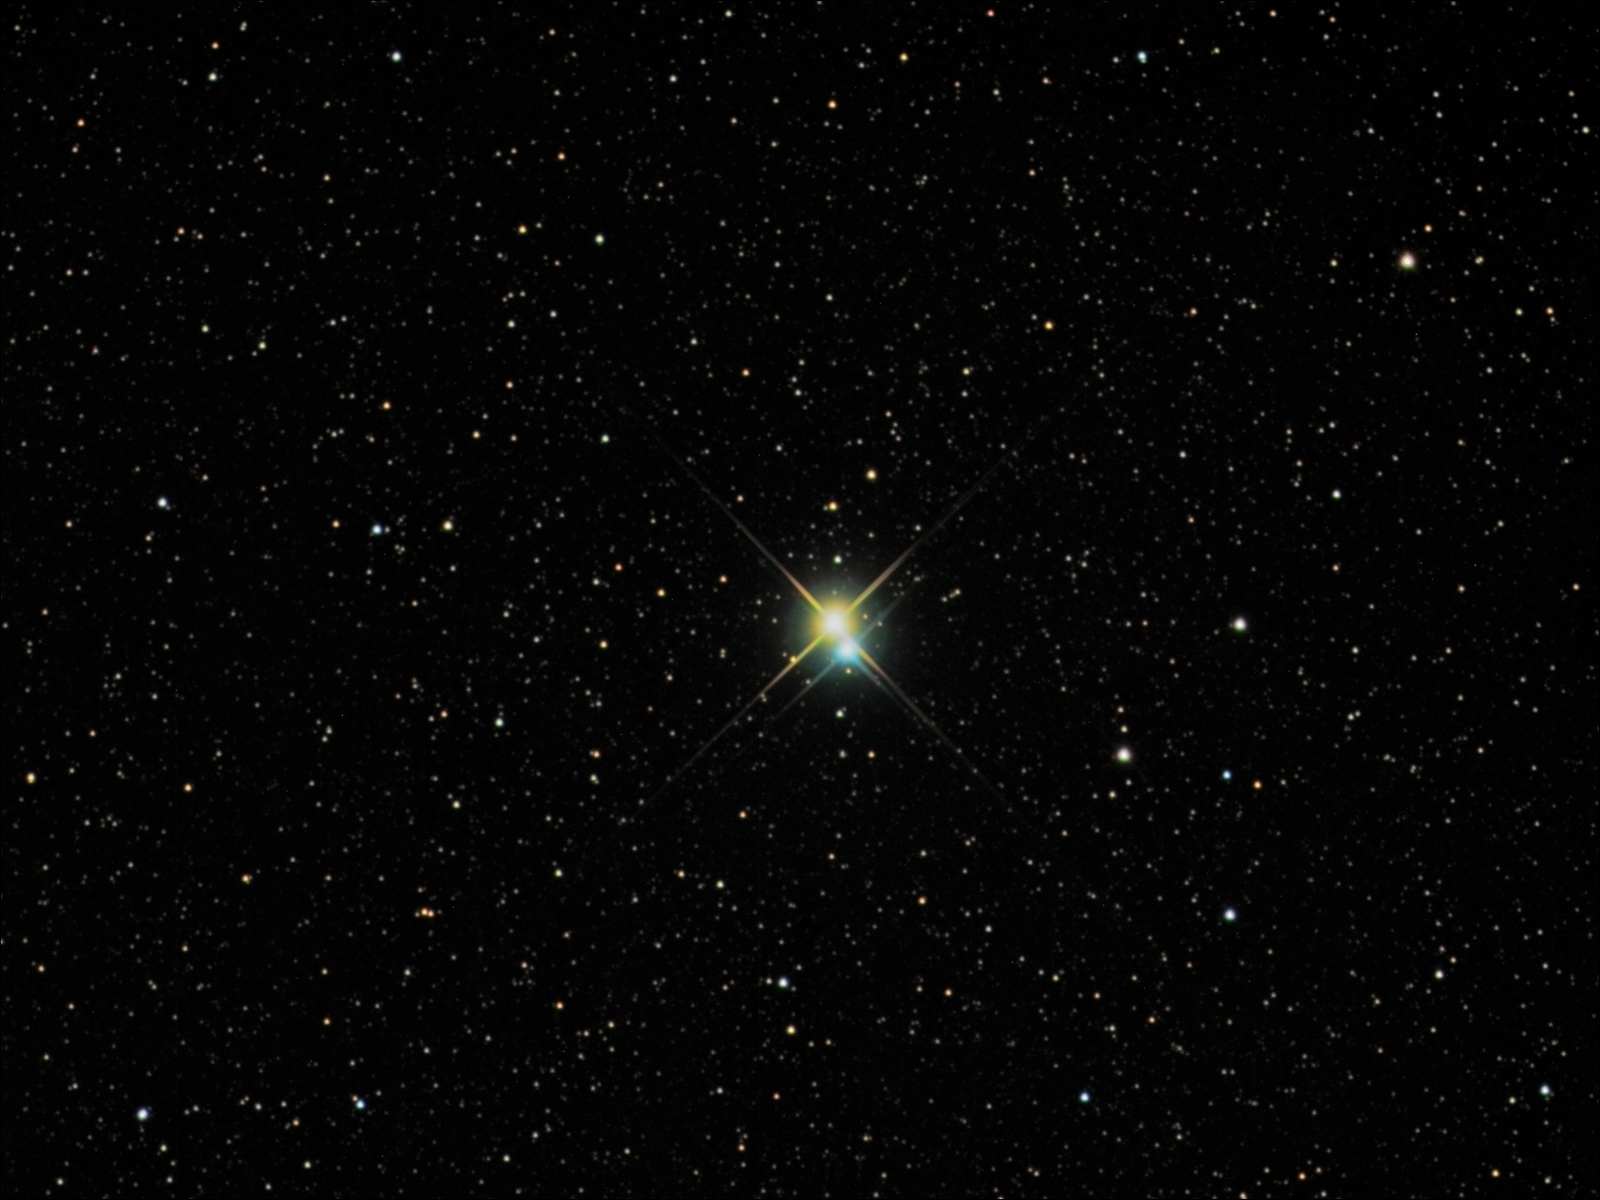
\includegraphics[width=\textwidth,trim=0 60 0 60,clip]{Albireo.jpg}
\caption{Albireo: A Bright and Beautiful Double. \emph{Credit \& Copyright: Richard Yandrick}.}
\label{fig:Albireo}
\end{figure}

\section{31 and 32 Cygni, \texorpdfstring{$\omicron^1$ and $\omicron^2$}{omicron1 and omicron2} Cygni}
\textbf{Type:} Multiple Star \\
\textbf{Magnitude:} 3.8, 4.0 \\
\textbf{Location Guide:} \textit{The two bright stars about 1/2
  between Deneb ($\alpha$ Cygni, ``tail'' of Cygnus) and Rukh
  ($\delta$ Cygni, middle of the left ``wing'' of Cygnus).}

The wide binary $\omicron^1$ Cygni and $\omicron^2$ Cygni is separated
61$'$ (NNE), and this star is an easy naked-eye double. $\omicron^1$
Cygni with 30 Cyg and HD 192579 (HIP 99676) is a moderately difficult
triple system. And surprise --- each of $\omicron^1$ Cyg and
$\omicron^2$ Cyg are also Algol-type eclipsing binaries!

\section{The Coathanger, Brocchi's Cluster, Cr 399}
\textbf{Type:} Asterism \\
\textbf{Location Guide:} \textit{It is best found by slowly sweeping
  across the Milky Way along an imaginary line from the bright star
  Altair toward the even brighter star Vega (around 1/3 between Altair
  and Vega).}

The asterism is made up of 10 stars ranging from 5th to 7th magnitude
which form the conspicuous ``coathanger'', a straight line of 6 stars
with a ``hook'' of 4 stars on the south side. Under a dark sky,
Collinder 399 can be seen with the naked eye as an unresolved patch of
light; binoculars or a telescope at very low power are usually needed
in order to view the ``coathanger'' asterism.

\section{Kemble's Cascade}
\textbf{Type:} Asterism \\
\textbf{Location Guide:} \textit{The asterism lies in the
  constellation Camelopardalis, about 1/3 between CS Cam and $\alpha$
  Cam --- HIP 18505 has magnitude 5 and can be found in the center of the
  chain.}

Kemble's Cascade is a chain of stars which are visible in binocular even
in light-polluted skies.

\section{The Double Cluster, \texorpdfstring{$\chi$ and \emph{h}}{chi and h} Persei, NGC 884 and NGC 869}
\textbf{Type:} Open Clusters \\
\textbf{Location Guide:} \textit{The two open clusters near stars $\chi$ and h in the constellation Perseus.}

The Double Cluster (also known as Caldwell 14 or C14) is the common
name for the naked-eye open clusters NGC 869 and NGC 884 (often
designated \emph{h} Persei and $\chi$ Persei, respectively). The
Double Cluster is approximately the radiant of the Perseid meteor
shower, which peaks annually around August 12 or 13. Although easy to
locate in the northern sky, observing the Double Cluster in its two
parts requires optical aid. They are described as being an
``awe-inspiring'' and ``breathtaking'' sight, and are often cited as 
targets in astronomical observers' guides.


\section{Large Magellanic Cloud, PGC 17223}
\textbf{Type:} Dwarf Spiral Galaxy \\
\textbf{Magnitude:} 0.9 \\
\textbf{Location Guide:} \textit{It is visible as a faint ``cloud'' in
  the night sky of the southern hemisphere straddling the border
  between the constellations of Dorado and Mensa, and it appears from
  Earth more than 20 times the width of the full moon.}

The \indexterm[Magellanic Cloud!Large]{Large Magellanic Cloud} (LMC) is a satellite galaxy of
the Milky Way. The Large Magellanic Cloud is usually considered an
irregular galaxy. However, it shows signs of a bar structure, and has more recently
been reclassified as a Magellanic-type dwarf spiral galaxy. At a
distance of 50 kiloparsecs, the LMC is the third closest galaxy to the
Milky Way, after the Sagittarius Dwarf Spheroidal (\textasciitilde16
kiloparsecs) and the putative Canis Major Dwarf Galaxy
(\textasciitilde12.9 kiloparsecs, though its status as a galaxy is
under dispute) lying closer to the center of the Milky Way. The LMC
has a diameter of about 14,000 light-years (\textasciitilde4.3 kpc)
and a mass of approximately 10 billion ($10^{10}$) solar
masses, making it roughly 1/100 as massive as the Milky Way. The LMC
has a wide range of galactic objects and phenomena --- surveys of the
galaxy have found roughly 60 globular clusters, 400 planetary nebulae,
and 700 open clusters, along with hundreds of thousands of giant and
supergiant stars.

\begin{figure}[ht]
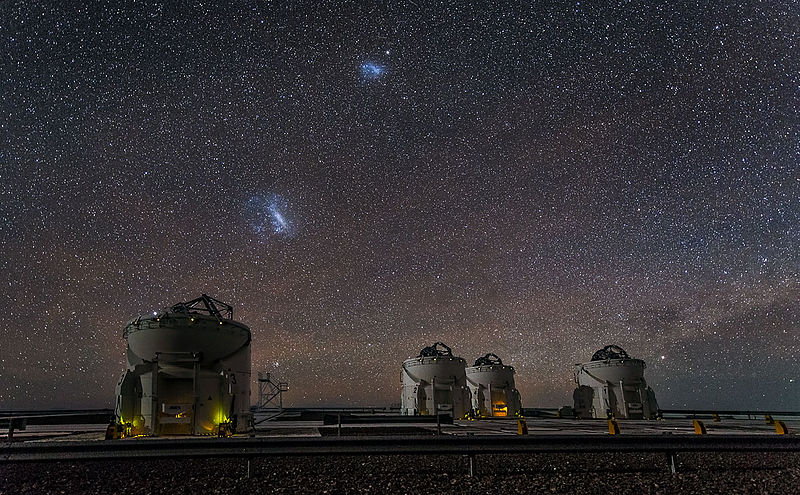
\includegraphics[width=\textwidth,trim=0 50 0 0,clip]{MagellanicClouds.jpg}
\caption{Small and Large Magellanic Clouds over Paranal Observatory. \emph{Credit: ESO/J. Colosimo}.}
\label{fig:MagellanicClouds}
\end{figure}

\section{Tarantula Nebula, C 103, NGC 2070}
\textbf{Type:} Nebula \\
\textbf{Magnitude:} 7.3 \\ 
\textbf{Location Guide:} \textit{Part of Large Magellanic Cloud.}

The Tarantula Nebula (also known as 30 Doradus) is an H II region in
the Large Magellanic Cloud (LMC). 30 Doradus has at its centre the
star cluster NGC 2070 which includes the compact concentration of
stars known as R136 that produces most of the energy that makes the
nebula visible. The estimated mass of the cluster is 450,000 solar
masses, suggesting it will likely become a globular cluster in the
future \cite{2009AJ....137.3437B}. The closest supernova observed
since the invention of the telescope, Supernova 1987A, occurred in the
outskirts of the Tarantula Nebula.

\section{Small Magellanic Cloud, NGC 292, PGC 3085}
\textbf{Type:} Dwarf Irregular Galaxy \\
\textbf{Magnitude:} 2.2 \\
\textbf{Location Guide:} \textit{It is located mostly in the
  constellation of Tucana and appears as a hazy, light patch in the
  night sky about 3$\degree$ across, looking like a detached piece of
  the Milky Way. Since it has a very low surface brightness, it is
  best viewed from a dark site away from city lights.}

The \indexterm[Magellanic Cloud!Small]{Small Magellanic Cloud} (SMC) is a dwarf galaxy near
the Milky Way. It is classified as a dwarf irregular galaxy. It has a
diameter of about 7,000 light-years and has a total mass of
approximately 7 billion times the mass of the Sun. The SMC contains a
central bar structure and it is speculated that it was once a barred
spiral galaxy that was disrupted by the Milky Way to become somewhat
irregular. At a distance of about 200,000 light-years, it is one of
the Milky Way's nearest neighbors. It is also one of the most distant
objects that can be seen with the naked eye.

\section{\texorpdfstring{$\omega$}{omega} Centauri cluster, C 80, NGC 5139}
\textbf{Type:} Globular Cluster \\
\textbf{Magnitude:} 5.3 \\ 
\textbf{Location Guide:} \textit{It is located around 1/3 between $\zeta$ and $\gamma$ Centauri.}

Omega Centauri ($\omega$ Cen), or NGC 5139, is a globular cluster in
the constellation of Centaurus that was first identified as a
non-stellar object by Edmond Halley in 1677. Located at a distance of
15,800 light-years (4,850 pc), it is the largest globular cluster in
the Milky Way at a diameter of roughly 150 light-years. It is
estimated to contain approximately 10 million stars and a total mass
equivalent to 4 million solar masses. Omega Centauri is so distinctive
from the other galactic globular clusters that it is thought to have
an alternate origin as the core remnant of a disrupted dwarf galaxy
\cite{2008ApJ...676.1008N}.

\section{47 Tucanae, C 106, NGC 104}
\textbf{Type:} Globular Cluster \\
\textbf{Magnitude:} 4.1 \\ 
\textbf{Location Guide:} \textit{It can be seen with the naked eye near Small Magellanic Cloud.}

It is the one of brightest globular cluster in the sky, and is noted
for having a very bright and dense core. It is also one of the most
massive globular clusters in the Milky Way Galaxy, containing millions of
stars. The cluster appears roughly the size of the full moon in the
sky under ideal conditions.

\section{The Coalsack Nebula, C 99}
\textbf{Type:} Dark Nebula \\
\textbf{Location Guide:} \textit{Dark region between $\alpha$ and $\beta$ Crux.}

The Coalsack Nebula is the most prominent dark nebula in the skies,
easily visible to the naked eye as a dark patch silhouetted against
the southern Milky Way. It is located at a distance of approximately
600 light years away from Earth. The Coalsack is important in
Australian Aboriginal astronomy, and forms the head of the Emu in the
sky in several Aboriginal cultures.

\begin{figure}[ht]
\centering
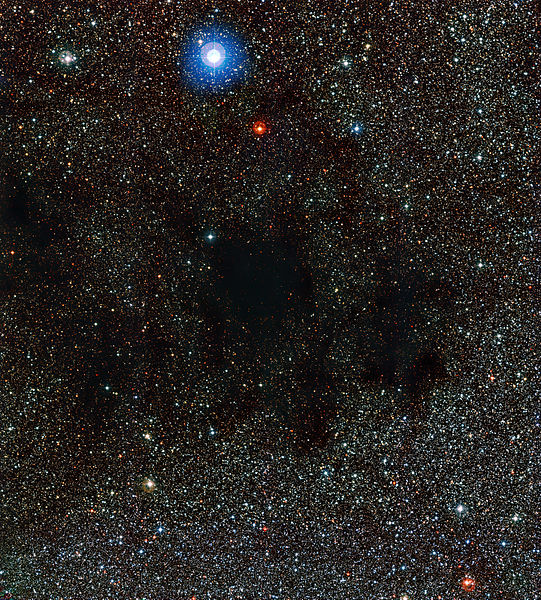
\includegraphics[width=0.65\textwidth]{CoalsackNebula.jpg}
\caption{The Coalsack Nebula taken by the Wide Field Imager on the MPG/ESO 2.2-metre telescope. \emph{Credit: ESO}.}
\label{fig:CoalsackNebula}
\end{figure}

\section{Mira, \texorpdfstring{$\omicron$}{omicron} Ceti, 68 Cet}
\textbf{Type:} Variable Star \\
\textbf{Magnitude:} 2.0--10.1 \\ 
\textbf{Location Guide:} \textit{It is located around 1/3 between $\delta$ and $\theta$ Ceti.}

Mira ($\omicron$ Ceti) is a star estimated 200--400 light years away
in the constellation Cetus. Mira is a binary star system that consists
of a red giant (Mira A) undergoing mass loss and a high temperature
white dwarf companion (Mira B) that is accreting mass from the
primary. Such an arrangement of stars is known as a symbiotic system,
and this is the closest such symbiotic pair to the Sun. Mira is the
brightest periodic variable in the sky that is not visible to the
naked eye for part of its cycle. Its distance is uncertain. Mira A is
a well-known example of a category of long-period variable stars known as Mira
variables, which are named after it.

\section{\texorpdfstring{$\alpha$}{alpha} Persei Cluster, Cr 39, Mel 20}
\textbf{Type:} Open Cluster \\
\textbf{Magnitude:} 1.2 \\ 
\textbf{Location Guide:} \textit{Around the white-yellow supergiant Mirfak, also known as $\alpha$ Persei in direction to $\delta$ Persei.}

The Alpha Persei Cluster, also known as Melotte 20 or Collinder 39, is
an open cluster in the constellation of Perseus. To the naked
eye, %% really NAKED EYE, or telescopic observer???
the cluster consists of several blue (spectral class B) stars.

\section{M7, The Ptolemy Cluster}
\textbf{Type:} Open Cluster \\
\textbf{Magnitude:} 3.3 \\
\textbf{Location Guide:} \textit{The cluster is easily detectable with
  the naked eye, close to the ``sting'' of Scorpius --- near the
  center of the line between Shaula ($\lambda$ Scorpii) and Kaus Media
  ($\delta$ Sagittarii).}

M7 has been known since antiquity --- it was first recorded by the
2nd-century Greek-Roman astronomer Ptolemy, who described it as a
nebula in 130 AD. Telescopic observations of the cluster reveal about
80 stars within a field of view of 1.3$\degree$ across. At the
cluster's estimated distance of 980 light years this corresponds to an
actual diameter of 25 light years.

\section{M24, The Sagittarius Star Cloud}
\textbf{Type:} Star Cloud \\
\textbf{Magnitude:} 4.6 \\ 
\textbf{Location Guide:} \textit{In the Milky Way region near Polis ($\mu$ Sagittarii).}

The Sagittarius Star Cloud is a star cloud in the constellation of
Sagittarius, approximately 600 light years wide. The stars, clusters
and other objects comprising M24 are part of the Sagittarius or
Sagittarius-Carina arms of the Milky Way galaxy. Messier described M24
as a ``large nebulosity containing many stars'' and gave its
dimensions as being some 1.5$\degree$ across.

\section{IC 4665, The Summer Beehive Cluster}
\textbf{Type:} Open Cluster \\
\textbf{Magnitude:} 4.2 \\ 
\textbf{Location Guide:} \textit{Visible to the naked eye near Cebalrai ($\beta$ Ophiuchi).}

IC 4665 is an open cluster in the constellation Ophiuchus which is
easily visible in the smallest of telescopes and also with
binoculars. From a sufficiently dark place it is also visible to the
naked eye.

\section{The E Nebula, Barnard 142 and 143}
\textbf{Type:} Dark Nebula \\
\textbf{Location Guide:} \textit{A well-defined dark area on a background of Milky Way near Tarazed ($\gamma$ Aquilae).}

The ``E'' or ``Barnard's E'' Nebula (officially designated as B142 and
B143) is a pair of dark nebulae in the constellation Aquila. It is a
well-defined dark area on a background of the Milky Way. The size of the
nebula is roughly 0.5$\degree$, and its distance from earth is
estimated at about 2000 light years.

%%% Local Variables: 
%%% mode: latex
%%% TeX-master: "guide"
%%% End: 
